\documentclass[10pt,a4paper]{report}
\usepackage[utf8]{inputenc}
\usepackage{amsmath}
\usepackage{amsfonts}
\usepackage{hyperref}
\usepackage{amssymb}
\usepackage{tikz-cd}
\usepackage {tikz}
\usepackage{lipsum}
\usetikzlibrary{arrows, positioning, automata}
\usetikzlibrary {positioning}
%\usepackage {xcolor}
\definecolor {processblue}{cmyk}{0.96,0,0,0}

\author{Salim Najib, Alexandre Sallinen}
\title{Rigel}
\begin{document}
\newcommand{\code}[1]{\texttt{#1}}
\section{Barre de recherche}

La barre de recherche permet à l'utilisateur de sélectionner un objet céleste pour la retrouver dans le ciel par son nom. A chaque lettre tapée, l'utilisateur voit une liste des objets célestes comencant par la même séquence de lettre que celle entrée. 

L'implémentation de cette barre de recherche passe par une classe abstraite qui représente une barre de recherche générale capable de fournir un objet (celui séléctionné au terme de la recherhce). Le \code{Searcher} constitue une implémentation de cette classe qui se spécialise dans les objets célestes. Pour éffectuer une recherche rapide, les noms des objets célestes sont entrés dans un arbre où chaque mot est décomposé par lettre et appartiennent à une même branche les mots qui ont une séquence de lettre identique à partir d'un certain indice.

\section{Parallélisme}

Afin d'améliorer la performance du programme, le \code{ThreadManager} génère un arbre de taches à éffectuer dans le main et asigne les taches dans le bon ordre à une réserve de threads.

Le principe de fonctionnement est le suivant : des annotations permettent au démarage de l'application de séparer le main en taches dépendantes les unes des autres. Pour notifier qu'une tache est dépendante d'une autre, l'annotation \code{Require} créée pour l'occasion, indique quels \textit{stages} auront du êtres complétés avant que ne soit éxécuté celui ci. Les tachent sont alors organisées dans un graphe, plus précisément une foret. Dans chaque arbre, les feuilles constituent les premières taches à effectuer. Les taches plus proches de la racine nécéssitent les précédentes avant d'être exécutées, c'est ce que défini l'annotation require. Le graphe suivant permet de mieux comprendre la situation :
\pagebreak
\begin{figure}
\centering
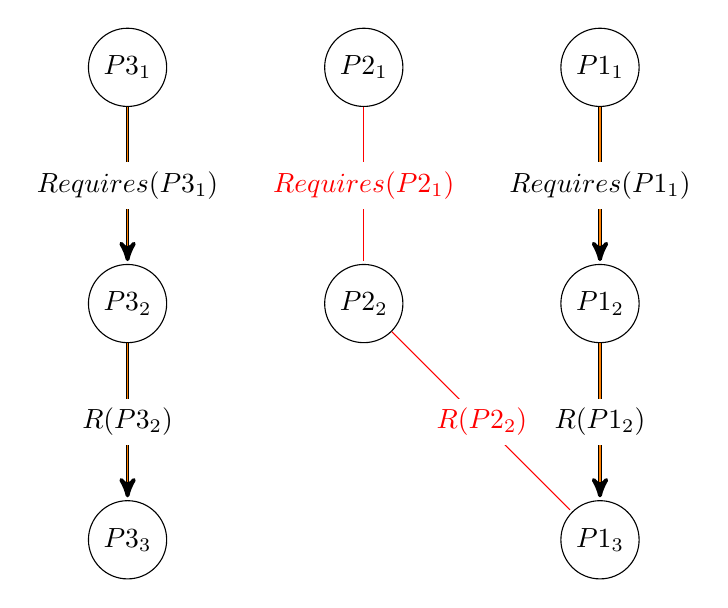
\begin{tikzpicture}[>=stealth',shorten >=1pt,node distance=3cm,on grid,initial/.style={}]

state/.style ={ circle ,top color =white , bottom color = processblue!20 ,
draw,processblue , text=blue , minimum width =1 cm}]

    \node[state] (P1) {$P1_1$};
    \node[state] (P2) [left  =of P1]{$P2_1$};
    \node[state] (P3) [left  =of P2]{$P3_1$};

    \node[state] (P12) [below =of P1] {$P1_2$};
    \node[state] (P22) [below =of P2] {$P2_2$};
    \node[state] (P13) [below =of P12] {$P1_3$};
    \node[state] (P32) [left =of P22] {$P3_2$};
    \node[state] (P33) [below =of P32] {$P3_3$};

    \tikzset{mystyle/.style={->,double=orange}}
    \tikzset{every node/.style={fill=white}}
    \path (P1)  edge  [mystyle] node {$Requires(P1_1)$} (P12);
    \path (P2)  edge  [red] node {$Requires(P2_1)$} (P22);
    \path (P3)  edge [mystyle] node {$Requires(P3_1)$} (P32);
    \path (P12) edge [mystyle] node {$R(P1_2)$} (P13);
    \path (P22) edge [red] node {$R(P2_2)$} (P13);
    \path (P32) edge [mystyle] node {$R(P3_2)$} (P33);

	

\end{tikzpicture}
\caption{Un graphe possible des taches}
\end{figure}

Chaque $PN_i$ représente un \textit{processus} qui sera éxécuté par le gestionnaire. En rouge une brache qui sera éxécuté par les mêmes threads en parallèle de ses branches adjacentes mais qui attendra la complétion de la branche des $P1_i$ pour continuer en $P1_3$. Ce système, quoique complexe, fait plein usage de la capacté des \code{Tree} définis dans le package graph et se montre très générale et réutilisable.


\section{Prédiction d'orbite}

La prédiction d'orbite permet de connaitre, en cliquant droit sur des planètes, leur position à venir. Ces futures positions sont modélisées par des points dont l'éspacement est réglable.

Ces orbites font plein usage du package graph en extendant les cycles, des arcs se refermant sur eux mêmes. Ainsi, l'orbite n'est qu'un cycle de \code{Supplier} pour limiter le calcul et ce sont les parametre d'espacement qui permettent de récupérer des positions à un intervale fixe de temps. L'intervalle fixe de temps permet graphiquement de représenté la vitesse d'un tel astre.  

\section{Géstion des paramètres d'interfaces graphique}

Le bouton labéllé avec un rouage à coté de la barre de recherche ouvre un paneau de réglages graphiques. En premier lieu, un mode \textit{cinématique} cachant l'interface utilisateur pour ne laisser que le ciel, une touche permettant d'activer ou de désactiver 
le \hyperref[sec:info]{paneau d'information} à volonté, un mode plein écran, et un bouton restreignant la vue au ciel réelement visible (interdiction d'observer sous la barre des $5^{\circ}$ d'hauteur). Ensuite, deux paramètres de sensibilités sont proposés. Pour finir, de nombreux paramètres graphiques gérant la couleur et les éléments à dessiner sont proposés. 

Le plein écran joue sur un simple paramètre du BorderPane (\code{setFullScreen}), le masquage du panneau de droite,la capacité à descendre plus bas et le mode cinématique sont modélisés par des propriétés booléenes misent en place dans le \code {main}.
Les sliders agissent quant à eux sur des valuers maximum et minimum definies dans le main. Enfin les paramètres dde couleurs et d'affichagess sont gérés de manière similaire, le \code{painter} ayant la capacité de changer la couleur de certains de ces éléments et les coches activant ou désactivant des parties du draw.




\section{Informations sur les corps célestes}
\label{sec:info}
La barre de droite du BorderPane affiche, lorsqu'un corps céleste est séléctionné, des propriétés intéréssante pour l'utilisateur qui souhaitera l'observer précisémet : Ses coordonées dans plusieurs systèmes, sa température et son hipparcos. Enfin ce panneau donnera aussi le nom de ses étoiles voisines dans l'astérisme.

L'implémentation de cette fonctionalité était aisée puisque les informations concernant un objet célèste sont dirèctement stocké en son sein.
Pour trouver les étoiles liées par un même astérisme, la méthode \code{constellationOfStar} fournit un getter pour la map \code{Map<Star, AbstractMathSet<Star>> constellationsMap} qui relis à chaque étoile, l'ensemble des étoiles lui étant reliées par un astérisme. La \code{Map} garantit un accès en $\mathcal{O}(1)$.
 

\end{document}